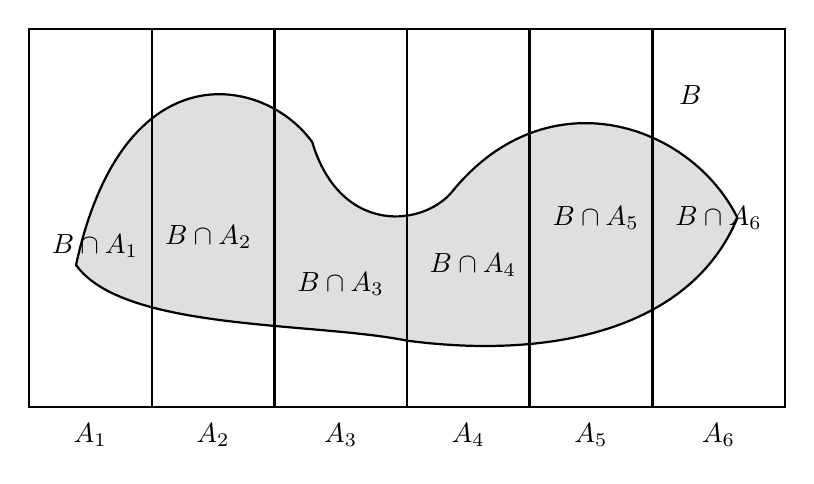
\begin{tikzpicture}[scale=1.2]

% Draw the sample space rectangle
\draw[thick] (0,0) rectangle (8,4);

% Label Ai regions
\node at (0.65,-0.3) {$A_1$};
\node at (1.95,-0.3) {$A_2$};
\node at (3.3,-0.3) {$A_3$};
\node at (4.65,-0.3) {$A_4$};
\node at (5.95,-0.3) {$A_5$};
\node at (7.3,-0.3) {$A_6$};

% Draw event B as an irregular shaded region
\filldraw[fill=gray!25, draw=black, line join=round, thick]
  (0.5,1.5) .. controls (1,3.8) and (2.5,3.5) .. (3,2.8)
  .. controls (3.3,1.8) and (4.2,1.9) .. (4.5,2.3)
  .. controls (5.5,3.5) and (7,3) .. (7.5,2)
  .. controls (7,0.8) and (5.5,0.5) .. (4,0.7)
  .. controls (3,0.9) and (1,0.8) .. (0.5,1.5) -- cycle;

% Draw partitions A1 to A6
\foreach \x in {0,1.3,2.6,4,5.3,6.6,8}
  \draw[thick] (\x,0) -- (\x,4);

% Label B region
\node at (7,3.3) {$B$};

% Label intersections B ∩ Ai
\node at (0.7,1.7) {$B\cap A_1$};
\node at (1.9,1.8) {$B\cap A_2$};
\node at (3.3,1.3) {$B\cap A_3$};
\node at (4.7,1.5) {$B\cap A_4$};
\node at (6.0,2.0) {$B\cap A_5$};
\node at (7.3,2.0) {$B\cap A_6$};

\end{tikzpicture}